\documentclass[aspectratio=169,11pt]{beamer}

\usepackage[T1]{fontenc}
\usepackage{amsmath,amssymb}
\usepackage{booktabs}
\usepackage{tikz}
\usetikzlibrary{arrows.meta,calc,positioning,shapes.geometric}

\definecolor{navy}{HTML}{102A43}
\definecolor{blue}{HTML}{1F5A94}
\definecolor{cyan}{HTML}{18A0AE}
\definecolor{gold}{HTML}{E7A93B}
\definecolor{red}{HTML}{C84B31}
\definecolor{green}{HTML}{2B8A6E}
\definecolor{ink}{HTML}{1B2430}
\definecolor{mist}{HTML}{EAF1F7}
\definecolor{softgray}{HTML}{66788A}

\setbeamercolor{normal text}{fg=ink,bg=white}
\setbeamercolor{structure}{fg=blue}
\setbeamercolor{frametitle}{fg=white,bg=navy}
\setbeamercolor{alerted text}{fg=red}
\setbeamercolor{block title}{fg=white,bg=blue}
\setbeamercolor{block body}{fg=ink,bg=mist}
\setbeamertemplate{navigation symbols}{}
\setbeamertemplate{itemize item}{\color{cyan}$\blacktriangleright$}
\setbeamertemplate{itemize subitem}{\color{blue}$\bullet$}
\setbeamertemplate{frametitle}{%
  \nointerlineskip
  \begin{beamercolorbox}[wd=\paperwidth,ht=0.72cm,dp=0.22cm,leftskip=0.45cm]{frametitle}
    \usebeamerfont{frametitle}\insertframetitle
  \end{beamercolorbox}}
\setbeamertemplate{footline}{%
  \leavevmode
  \hbox{%
    \begin{beamercolorbox}[wd=.82\paperwidth,ht=2.6ex,dp=1.1ex,leftskip=.45cm]{author in head/foot}%
      \color{softgray}\scriptsize Assured PNT, Part 1: Navigation When GPS Cannot Be Trusted
    \end{beamercolorbox}%
    \begin{beamercolorbox}[wd=.18\paperwidth,ht=2.6ex,dp=1.1ex,rightskip=.45cm plus1fil]{date in head/foot}%
      \color{softgray}\scriptsize \insertframenumber/\inserttotalframenumber
    \end{beamercolorbox}}}

\newcommand{\source}[1]{\vfill\hfill{\color{softgray}\tiny Source: #1}}
\newcommand{\keyterm}[1]{\textcolor{blue}{\textbf{#1}}}
\newcommand{\pill}[2]{%
  \tikz[baseline=(p.base)]\node[rounded corners=3pt,fill=#1!13,draw=#1!65,
    inner xsep=6pt,inner ysep=3pt] (p) {\color{ink}\strut #2};}

\title{Assured PNT}
\subtitle{Navigation When GPS Cannot Be Trusted}
\author{Michael L. Carroll}
\date{2026}

\begin{document}

\begin{frame}[plain]
  \begin{tikzpicture}[remember picture,overlay]
    \fill[navy] (current page.south west) rectangle (current page.north east);
    \fill[cyan] (current page.south west) rectangle ([xshift=.18cm]current page.north west);
    \node[anchor=west,text width=9.4cm] at ([xshift=1.15cm,yshift=.75cm]current page.west) {
      {\color{white}\Huge\textbf{Assured PNT}}\\[0.25cm]
      {\color{white}\LARGE Navigation When GPS Cannot Be Trusted}\\[0.55cm]
      {\color{mist}\large Michael L. Carroll}\\[-0.02cm]
      {\color{mist}\small Kalman Filter Theory and Applications}};
    \node[circle,draw=cyan,line width=1.2pt,text=white,minimum size=1.45cm]
      (p) at ([xshift=-3.3cm,yshift=.65cm]current page.east) {\Large P};
    \node[circle,draw=gold,line width=1.2pt,text=white,minimum size=1.45cm]
      (n) at ([xshift=-1.75cm,yshift=.65cm]current page.east) {\Large N};
    \node[circle,draw=green,line width=1.2pt,text=white,minimum size=1.45cm]
      (t) at ([xshift=-2.52cm,yshift=-.85cm]current page.east) {\Large T};
    \draw[cyan!80,line width=1pt] (p)--(n)--(t)--cycle;
  \end{tikzpicture}
\end{frame}

\begin{frame}{A confident answer can still be wrong}
  \begin{columns}[T,onlytextwidth]
    \column{.56\textwidth}
      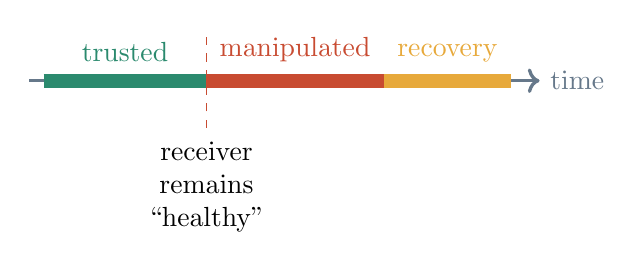
\begin{tikzpicture}[x=.9cm,y=1cm]
        \draw[->,line width=1.2pt,softgray] (0,0) -- (7.2,0) node[right] {time};
        \draw[line width=5pt,green] (.2,0) -- (2.5,0);
        \draw[line width=5pt,red] (2.5,0) -- (5.0,0);
        \draw[line width=5pt,gold] (5.0,0) -- (6.8,0);
        \node[above,green] at (1.35,.12) {trusted};
        \node[above,red] at (3.75,.12) {manipulated};
        \node[above,gold] at (5.9,.12) {recovery};
        \draw[dashed,red] (2.5,-.6)--(2.5,.65);
        \node[below,text width=2.2cm,align=center] at (2.5,-.65)
          {receiver remains ``healthy''};
      \end{tikzpicture}
      \vspace{0.35cm}
      \begin{block}{The dangerous case}
        The navigation computer continues to report a precise solution while
        the external measurement has become misleading.
      \end{block}
    \column{.40\textwidth}
      \pause
      \Large
      \begin{itemize}
        \item Availability is not integrity.
        \item Precision is not truth.
        \item Fusion is not automatic trust.
      \end{itemize}
  \end{columns}
  \source{FAA, \emph{GNSS Interference Resource Guide}, 2025}
\end{frame}

\begin{frame}{What PNT provides}
  \centering
  
\begin{tikzpicture}[node distance=.55cm]
    \uncover<1->{\node[rounded corners=8pt,draw=blue,fill=blue!9,minimum width=3.5cm,
      minimum height=3.0cm,align=center] (p) {\color{blue}\Huge P\\[.15cm]
      \large\textbf{Position}\\[-.02cm]\small Where am I?};}
    \uncover<2->{\node[rounded corners=8pt,draw=cyan,fill=cyan!9,minimum width=3.5cm,
      minimum height=3.0cm,align=center,right=of p] (n) {\color{cyan}\Huge N\\[.15cm]
      \large\textbf{Navigation}\\[-.02cm]\small Where am I going?};}
    \uncover<3->{\node[rounded corners=8pt,draw=gold,fill=gold!10,minimum width=3.5cm,
      minimum height=3.0cm,align=center,right=of n] (t) {\color{gold!80!black}\Huge T\\[.15cm]
      \large\textbf{Timing}\\[-.02cm]\small When did it happen?};}
  \end{tikzpicture}

  \uncover<4->{\vspace{.45cm}
    \large A resilient system must preserve the \textbf{mission-relevant combination}
    of position, velocity, attitude, and time.}
\end{frame}

\begin{frame}{GPS is powerful---and physically fragile}
  \begin{columns}[T,onlytextwidth]
    \column{.48\textwidth}
      \begin{block}{Why we use it}
        \begin{itemize}
          \item Global, common reference
          \item Position, velocity, and precise time
          \item Excellent long-term stability
          \item Low user-equipment burden
        \end{itemize}
      \end{block}
    \column{.48\textwidth}
      \pause
      \begin{alertblock}{Why it needs help}
        \begin{itemize}
          \item Very low received signal power
          \item Blockage, multipath, and interference
          \item Jamming can remove measurements
          \item Spoofing can create plausible false data
        \end{itemize}
      \end{alertblock}
  \end{columns}
  \uncover<3->{\vspace{.25cm}\centering\Large
    Design for \textbf{loss} and \textbf{manipulation}, not merely nominal accuracy.}
  \source{GPS.gov resilience guidance; FAA GNSS Interference Resource Guide}
\end{frame}

\begin{frame}{Two failures, two different hazards}
  \begin{columns}[T,onlytextwidth]
    \column{.47\textwidth}
      \begin{block}{Jamming: deny the signal}
        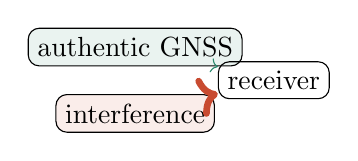
\begin{tikzpicture}[node distance=.35cm]
          \node[draw,rounded corners,fill=green!10] (sat) {authentic GNSS};
          \node[draw,rounded corners,fill=red!10,below=of sat] (jam) {interference};
          \node[draw,rounded corners,right=1.05cm of $(sat)!0.5!(jam)$] (rx) {receiver};
          \draw[->,green] (sat)--(rx);
          \draw[->,red,line width=2.4pt] (jam)--(rx);
        \end{tikzpicture}
        \begin{itemize}
          \item The authentic signal is overwhelmed.
          \item Loss or degradation may be obvious.
        \end{itemize}
      \end{block}
    \column{.47\textwidth}
      \pause
      \begin{alertblock}{Spoofing: counterfeit the signal}
        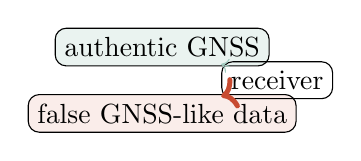
\begin{tikzpicture}[node distance=.35cm]
          \node[draw,rounded corners,fill=green!10] (sat) {authentic GNSS};
          \node[draw,rounded corners,fill=red!10,below=of sat] (spoof) {false GNSS-like data};
          \node[draw,rounded corners,right=.75cm of $(sat)!0.5!(spoof)$] (rx) {receiver};
          \draw[->,green!45] (sat)--(rx);
          \draw[->,red,line width=1.8pt] (spoof)--(rx);
        \end{tikzpicture}
        \begin{itemize}
          \item The false signal looks plausible.
          \item Bad data can contaminate fused systems.
        \end{itemize}
      \end{alertblock}
  \end{columns}
  \uncover<3->{\centering\small A Kalman filter can reject inconsistent data;
    it does not, by itself, authenticate GNSS.}
  \source{FAA, \emph{GNSS Interference Resource Guide}, Sections 1.5--1.7}
\end{frame}

\begin{frame}{Assurance is a behavior, not a sensor}
  \centering
  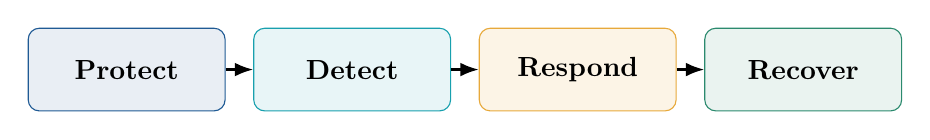
\begin{tikzpicture}[node distance=.35cm,>=Latex]
    \uncover<1->{\node[rounded corners,draw=blue,fill=blue!10,minimum width=2.5cm,
      minimum height=1.05cm] (protect) {\textbf{Protect}};}
    \uncover<2->{\node[rounded corners,draw=cyan,fill=cyan!10,minimum width=2.5cm,
      minimum height=1.05cm,right=of protect] (detect) {\textbf{Detect}};
      \draw[->,thick] (protect)--(detect);}
    \uncover<3->{\node[rounded corners,draw=gold,fill=gold!13,minimum width=2.5cm,
      minimum height=1.05cm,right=of detect] (respond) {\textbf{Respond}};
      \draw[->,thick] (detect)--(respond);}
    \uncover<4->{\node[rounded corners,draw=green,fill=green!10,minimum width=2.5cm,
      minimum height=1.05cm,right=of respond] (recover) {\textbf{Recover}};
      \draw[->,thick] (respond)--(recover);}
  \end{tikzpicture}

  \uncover<5->{\vspace{.5cm}
  \begin{columns}[T,onlytextwidth]
    \column{.23\textwidth}\centering Prevent avoidable exposure
    \column{.23\textwidth}\centering Recognize anomalies quickly
    \column{.23\textwidth}\centering Continue at known performance
    \column{.23\textwidth}\centering Re-admit sources safely
  \end{columns}}

  \uncover<6->{\vspace{.5cm}\large
    \pill{navy}{The system must know what it trusts---and why.}}
  \source{NIST IR 8323 Rev. 1; DHS Resilient PNT Reference Architecture}
\end{frame}

\begin{frame}{Inertial navigation provides the bridge}
  \begin{columns}[T,onlytextwidth]
    \column{.48\textwidth}
      \begin{block}{INS strengths}
        \begin{itemize}
          \item Self-contained after initialization
          \item High-rate position, velocity, and attitude
          \item Immune to radio-frequency jamming
          \item Smooth short-term propagation
        \end{itemize}
      \end{block}
    \column{.48\textwidth}
      \pause
      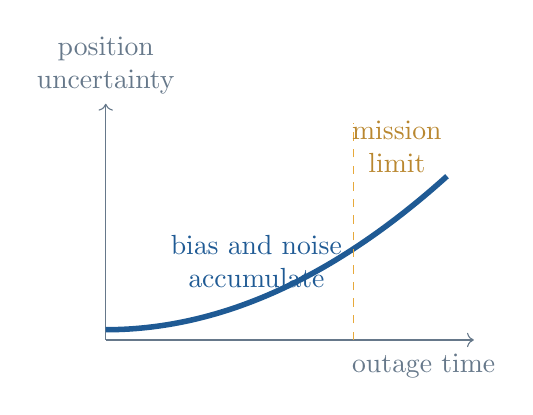
\begin{tikzpicture}[x=.85cm,y=1cm]
        \draw[->,softgray] (0,0)--(5.5,0);
        \node[below,softgray] at (4.75,-.05) {outage time};
        \draw[->,softgray] (0,0)--(0,3.0) node[above,align=center] {position\\uncertainty};
        \draw[blue,line width=2pt,domain=0:5.1,samples=60]
          plot (\x,{0.13+0.075*\x*\x});
        \draw[dashed,gold] (3.7,0)--(3.7,2.75);
        \node[align=center,gold!80!black] at (4.35,2.45) {mission\\limit};
        \node[align=center,blue] at (2.25,1.0) {bias and noise\\accumulate};
      \end{tikzpicture}
      \begin{alertblock}{INS limitation}
        Without trusted aiding, uncertainty grows and the solution eventually
        exceeds the mission's error bound.
      \end{alertblock}
  \end{columns}
\end{frame}

\begin{frame}{Resilience comes from complementary errors}
  \centering
  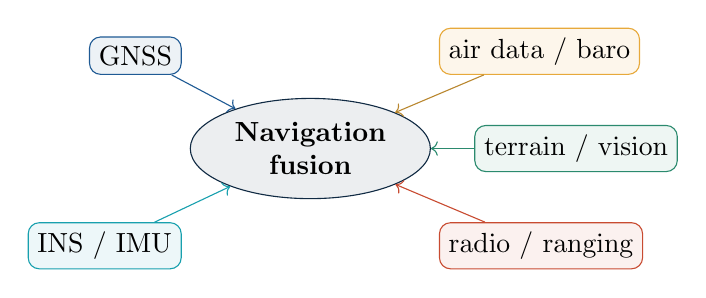
\begin{tikzpicture}[node distance=.48cm and .55cm]
    \node[ellipse,draw=navy,fill=navy!8,minimum width=3.0cm,minimum height=1.2cm,
      align=center] (fusion) {\textbf{Navigation}\\\textbf{fusion}};
    \uncover<1->{\node[rounded corners,draw=blue,fill=blue!8,above left=of fusion] (gnss)
      {GNSS}; \draw[->,blue] (gnss)--(fusion);}
    \uncover<1->{\node[rounded corners,draw=cyan,fill=cyan!8,below left=of fusion] (ins)
      {INS / IMU}; \draw[->,cyan] (ins)--(fusion);}
    \uncover<2->{\node[rounded corners,draw=gold,fill=gold!10,above right=of fusion] (air)
      {air data / baro}; \draw[->,gold!80!black] (air)--(fusion);}
    \uncover<2->{\node[rounded corners,draw=green,fill=green!8,right=of fusion] (terrain)
      {terrain / vision}; \draw[->,green] (terrain)--(fusion);}
    \uncover<2->{\node[rounded corners,draw=red,fill=red!8,below right=of fusion] (radio)
      {radio / ranging}; \draw[->,red] (radio)--(fusion);}
  \end{tikzpicture}

  \uncover<3->{\vspace{.55cm}
    \begin{block}{The design test}
      Sources are valuable when their failure modes are sufficiently independent
      and their measurements make the needed states observable.
    \end{block}}
  \source{U.S. DOT Complementary PNT Action Plan, 2024}
\end{frame}

\begin{frame}{The Kalman filter is the integration engine}
  \centering
  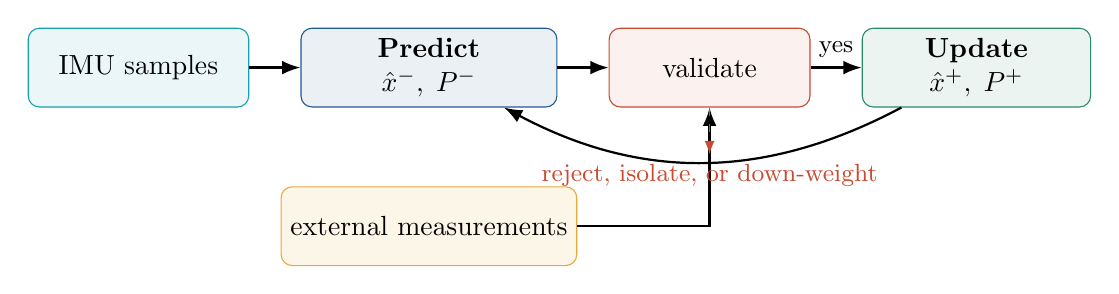
\begin{tikzpicture}[node distance=.42cm and .65cm,>=Latex]
    \node[rounded corners,draw=cyan,fill=cyan!9,minimum width=2.8cm,minimum height=1cm]
      (imu) {IMU samples};
    \node[rounded corners,draw=blue,fill=blue!9,minimum width=3.25cm,minimum height=1cm,
      align=center,
      right=of imu] (predict) {\textbf{Predict}\\$\hat{x}^{-},\;P^{-}$};
    \node[rounded corners,draw=gold,fill=gold!11,minimum width=3.0cm,minimum height=1cm,
      below=1.0cm of predict] (measure) {external measurements};
    \node[rounded corners,draw=red,fill=red!8,minimum width=2.55cm,
      minimum height=1cm,right=of predict] (gate) {validate};
    \node[rounded corners,draw=green,fill=green!9,minimum width=2.9cm,minimum height=1cm,
      align=center,
      right=of gate] (update) {\textbf{Update}\\$\hat{x}^{+},\;P^{+}$};
    \draw[->,thick] (imu)--(predict);
    \draw[->,thick] (predict)--(gate);
    \draw[->,thick] (measure)-| (gate);
    \draw[->,thick] (gate)--node[above,font=\small]{yes}(update);
    \draw[->,thick] (update) to[bend left=28] (predict);
    \draw[->,red,dashed] (gate) -- ++(0,-1.1)
      node[below,font=\small] {reject, isolate, or down-weight};
  \end{tikzpicture}

  \vspace{.35cm}
  \keyterm{Prediction} carries the solution through gaps.\qquad
  \keyterm{Updates} bound drift---only when they are trustworthy.
\end{frame}

\begin{frame}{A practical error-state model}
  \centering
  \uncover<1->{\[
    \delta x =
    \begin{bmatrix}
      \delta r & \delta v & \delta \theta & b_a & b_g & b_c & d_c
    \end{bmatrix}^{\!T}
  \]}
  \vspace{-.15cm}
  \uncover<2->{
  \begin{tabular}{@{}lll@{}}
    \toprule
    Group & Meaning & Why estimate it? \\
    \midrule
    $\delta r,\delta v$ & position and velocity errors & navigation output \\
    $\delta\theta$ & small attitude errors & correct force projection \\
    $b_a,b_g$ & accelerometer and gyro biases & control inertial drift \\
    $b_c,d_c$ & clock bias and drift & align measurements in time \\
    \bottomrule
  \end{tabular}}

  \uncover<3->{\vspace{.45cm}
    \pill{cyan}{The state is a design choice: estimate what the mission must control.}}
\end{frame}

\begin{frame}{Trust begins with the innovation}
  \begin{columns}[T,onlytextwidth]
    \column{.48\textwidth}
      \uncover<1->{\[
        \nu_k = z_k - h\!\left(\hat{x}^{-}_k\right)
      \]}
      \centering The innovation asks: \emph{What did the sensor say that the
      predicted state did not expect?}
      \uncover<2->{\[
        \mathrm{NIS}_k = \nu_k^T S_k^{-1}\nu_k
      \]}
    \column{.48\textwidth}
      \uncover<3->{
      \begin{block}{Before accepting an update}
        \begin{itemize}
          \item Check statistical consistency.
          \item Compare independent sources.
          \item Monitor signal and receiver health.
          \item Apply persistence and recovery logic.
        \end{itemize}
      \end{block}}
  \end{columns}
  \uncover<4->{\centering\large
    A residual gate is evidence of inconsistency---not proof of the cause.}
\end{frame}

\begin{frame}{What the system should do during an outage}
  \centering
  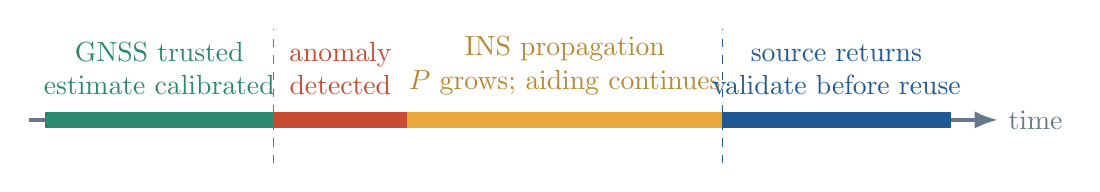
\begin{tikzpicture}[x=1cm,y=1cm,>=Latex]
    \draw[->,line width=1.2pt,softgray] (.2,0)--(12.5,0) node[right]{time};
    \uncover<1->{
      \draw[line width=6pt,green] (.4,0)--(3.3,0);
      \node[above,align=center,green] at (1.85,.2) {GNSS trusted\\estimate calibrated};}
    \uncover<2->{
      \draw[line width=6pt,red] (3.3,0)--(5.0,0);
      \node[above,align=center,red] at (4.15,.2) {anomaly\\detected};
      \draw[dashed,red] (3.3,-.55)--(3.3,1.15);}
    \uncover<3->{
      \draw[line width=6pt,gold] (5.0,0)--(9.0,0);
      \node[above,align=center,gold!80!black] at (7.0,.2) {INS propagation\\$P$ grows; aiding continues};}
    \uncover<4->{
      \draw[line width=6pt,blue] (9.0,0)--(11.9,0);
      \node[above,align=center,blue] at (10.45,.2) {source returns\\validate before reuse};
      \draw[dashed,blue] (9.0,-.55)--(9.0,1.15);}
  \end{tikzpicture}

  \uncover<5->{\vspace{.55cm}
    \begin{block}{Graceful degradation}
      Continue the mission only while the estimated uncertainty remains inside
      a declared operational limit; otherwise transition to a safe mode.
    \end{block}}
\end{frame}

\begin{frame}{Four design rules for assured PNT}
  \begin{enumerate}
    \setlength{\itemsep}{.35cm}
    \uncover<1->{\item \keyterm{Diversify}: combine sources with different physics and failure modes.}
    \uncover<2->{\item \keyterm{Manage trust}: never equate a precise measurement with an authentic one.}
    \uncover<3->{\item \keyterm{Expose uncertainty}: propagate covariance and compare it with mission limits.}
    \uncover<4->{\item \keyterm{Plan recovery}: define how sources are isolated, tested, and safely re-admitted.}
  \end{enumerate}

  \uncover<5->{\vspace{.35cm}\centering\Large
    \textbf{Assurance is the controlled behavior of the whole system.}}
  \source{DHS Resilient PNT Reference Architecture; DHS RPNT Best Practices, 2025}
\end{frame}

\begin{frame}{The central idea}
  \centering
  \Large
  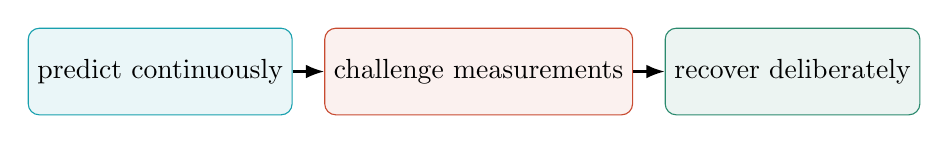
\begin{tikzpicture}[node distance=.40cm,>=Latex,font=\normalsize]
    \node[rounded corners,draw=cyan,fill=cyan!9,minimum width=2.85cm,minimum height=1.1cm]
      (predict) {predict continuously};
    \node[rounded corners,draw=red,fill=red!8,minimum width=2.85cm,minimum height=1.1cm,
      right=of predict] (challenge) {challenge measurements};
    \node[rounded corners,draw=green,fill=green!9,minimum width=2.85cm,minimum height=1.1cm,
      right=of challenge] (recover) {recover deliberately};
    \draw[->,thick] (predict)--(challenge);
    \draw[->,thick] (challenge)--(recover);
  \end{tikzpicture}

  \vspace{.75cm}
  \textbf{A resilient navigator does not promise perfect availability.}\\[.15cm]
  It promises known performance, visible uncertainty, and safe behavior.

  \vspace{.6cm}
  \normalsize Next: alternative aiding sources and terrain-referenced navigation.
\end{frame}

\begin{frame}{Primary references}
  \small
  \begin{thebibliography}{9}
    \bibitem{FAA2025}
      Federal Aviation Administration,
      \emph{GPS and GNSS Interference Resource Guide}, 2025.\\
      \url{https://www.faa.gov/about/office_org/headquarters_offices/avs/offices/afx/afs400/afs410/GNSS}
    \bibitem{GPSGov}
      GPS.gov, \emph{Resilience Through Responsible Use of PNT}.\\
      \url{https://www.gps.gov/resilience-through-responsible-use-pnt}
    \bibitem{NIST8323}
      NIST IR 8323 Rev. 1, \emph{Foundational PNT Profile}, 2023.\\
      \url{https://doi.org/10.6028/NIST.IR.8323r1}
    \bibitem{DHSRA}
      DHS, \emph{Resilient PNT Reference Architecture}, 2022.\\
      \url{https://www.dhs.gov/sites/default/files/2022-06/22_0609_st_resilient_pnt_ra.pdf}
    \bibitem{DOT2024}
      U.S. DOT, \emph{Complementary PNT Action Plan}, 2024.\\
      \url{https://www.transportation.gov/pnt/complementary-pnt-action-plan}
    \bibitem{DHS2025}
      DHS, \emph{Best Practices for Resilient PNT Supporting Critical Infrastructure}, 2025.
  \end{thebibliography}
\end{frame}

\end{document}
